\begin{figure}[t]
\centering

\begin{subfigure}{\linewidth}
    \centering
    \makebox[\linewidth][c]{%
        
\includegraphics[width=1.25\linewidth]{plots/toksuite/dose_response_grid_pooled.pdf}
    }
    \caption{Toksuite models}
    \label{fig:toksuite_stacked}
\end{subfigure}

\vspace{0.75em}

\begin{subfigure}{\linewidth}
    \centering
    \makebox[\linewidth][c]{%
        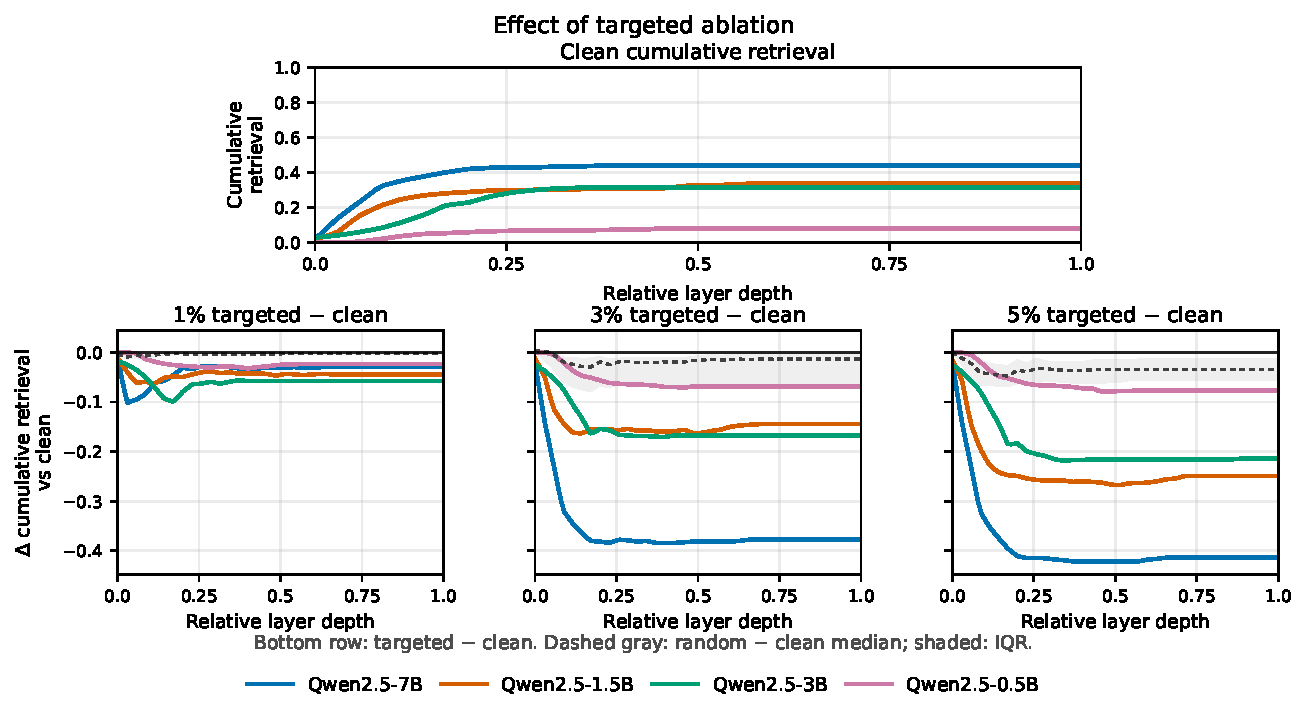
\includegraphics[width=1.25\linewidth]{plots/qwen/dose_response_grid_pooled.pdf}
    }
    \caption{\texttt{qwen2.5}}
    \label{fig:qwen_stacked}
\end{subfigure}

\caption[Layerwise cumulative retrieval across model families]{Cumulative retrieval under targeted ablation, pooled across languages. The top panel shows the clean baseline. The bottom row shows targeted minus clean at increasing ablation levels, with random ablation shown as median and interquartile range. More negative values indicate stronger disruption, while recovery at later layers reflects later compensation.}
\label{fig:ablation_stacked}
\end{figure}
